\documentclass{article}
\usepackage[utf8]{inputenc}
\usepackage{natbib}
\usepackage{graphicx}
\usepackage{hyperref}
\title{Laporan Harian Proyek 1}
\author{Burhanudin Zuhri}
\date{April 2020}
\begin{document}

\maketitle
	\begin{center}
		
\includegraphics[width=8cm,height=8cm]{logo.png}
	\end{center}
	\vspace{0.5 cm}
	
	\begin{center}
		Burhanudin Zuhri \\
		1194008 \\
		1A D4 TI \linebreak
		\newline
		\newline
		\newline
		\linebreak
		\newline
		\newline
		PROGRAM STUDI D4 TEKNIK INFORMATIKA \\
		POLITEKNIK POS INDONESIA\\
		2019/2020\\
	\end{center}

\section{Tanggal 26 Maret 2020:}
\newline
Pada tanggal ini kami bergabung dengan grup bimbingan Mr. Awangga. Kami mendapat tugas pertama kami untuk menginstall navicat dan terkoneksi dengan database MySQL. Besoknya kami diberi tugas untuk mengisi tabel notfound_message dan error_message dengan persetujuan setiap kelompok memilih salah satu tabel tersebut. Serta setiap orang dari dari masing-masing kelompok harus mengisi 100 record. . Berikut merupakan langkah mendownload dan menginstal Navicat:
\newline
\begin{enumerate}
        \item 1. Untuk menginstal \textbf{Navicat} kami mengunduh dahulu di internet di \textbf{website} resmi \textbf{Navicat}.
        \newline
        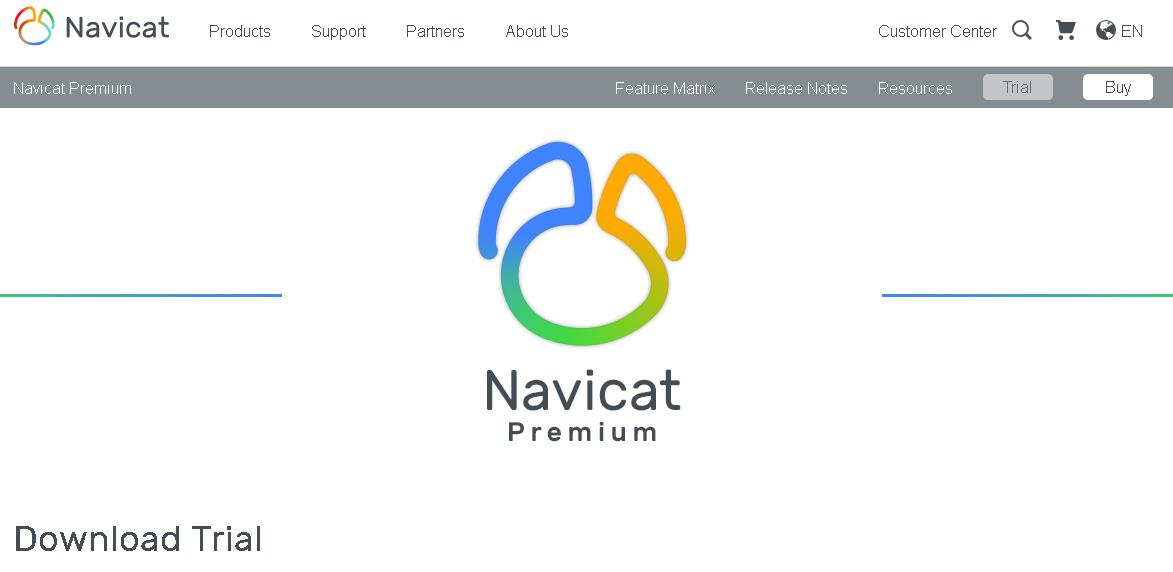
\includegraphics[scale=0.3]{26.1.jpg}
        \newline
        \item 2. Kami memilih \textbf{Navicat} yang sesuai dengan spesifikasi laptop kami.
        \newline
        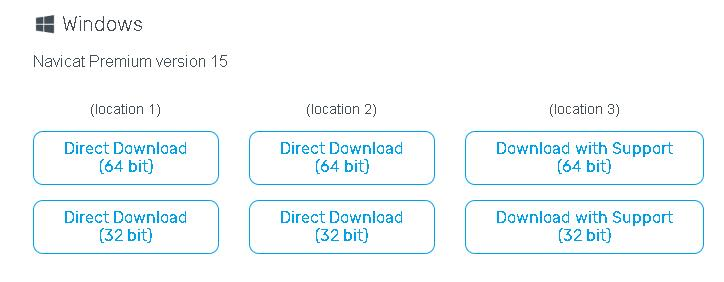
\includegraphics[scale=0.5]{26.2.jpg}
        \newline
        \item 3. Setelah \textbf{Navicat} selesai diunduh, maka selanjutnya kami menginstal \textbf{Navicat}
        \newline
        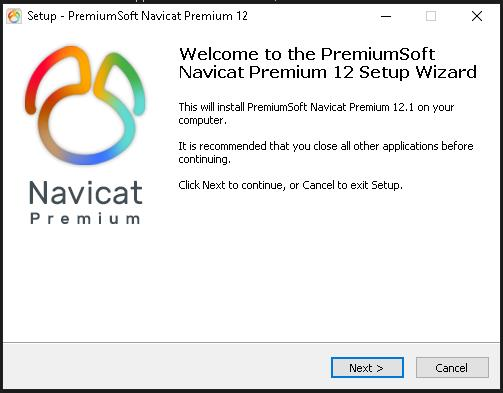
\includegraphics[scale=0.5]{26.3.jpg}
        \newline
        \item 4. Jika \textbf{Navicat} sudah diinstal selanjutnya yaitu mengaktifkan \textbf{database} \textbf{MySQL} pada aplikasi \textbf{XAMPP} agar servis \textbf{MySQL} dapat berjalan
         \newline
        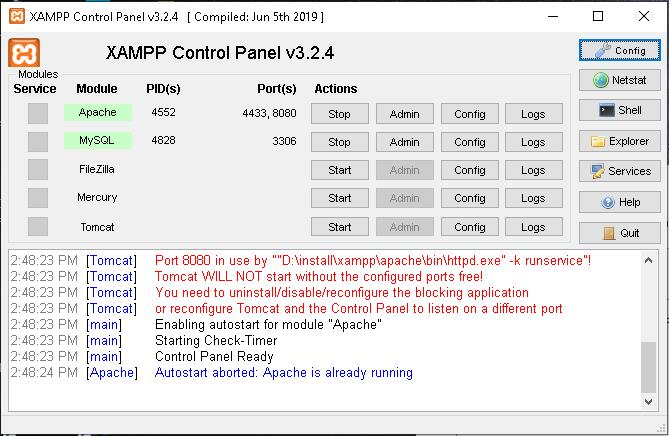
\includegraphics[scale=0.4]{26.4.jpg}
        \newline
        \item 5. Mengerjakan tugas \textbf{error_message} dan berhubung pada hari tersebut belum dapat menginputkan record pada database “bimbingan” maka kami menululiskan dahulu di \textbf{database} \textbf{MySQL}.
        \newline
        \newline
        a. Membuat koneksi  dengan cara menekan tombol icon Connection pada bagian kiri atas Navicat 
         \newline
        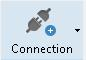
\includegraphics[scale=2]{26.5a.jpg}
        \newline
        b. Mengatur  host name,  port,  unsername, dan password MySQL
          \newline
        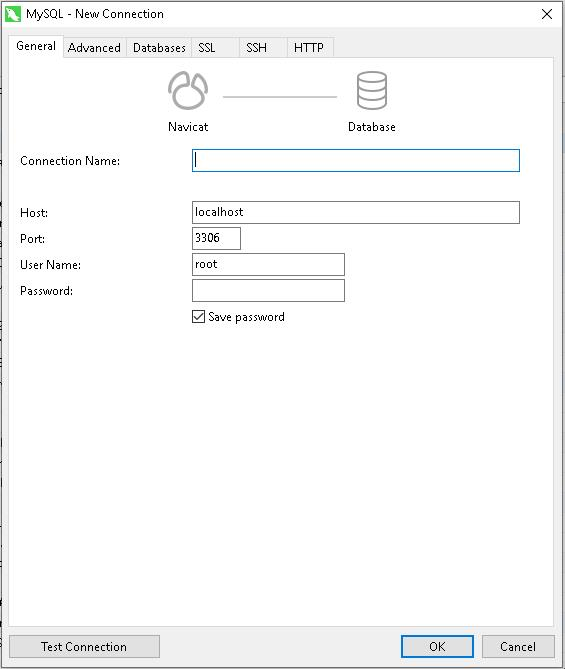
\includegraphics[scale=0.5]{26.5b.jpg}
        \newline
        c. Membuat databse baru dengan cara klik kanan padaMySQL dan pilih New Database lalu isi dengan nama bebas (disini saya menamainya dengan nama content_chatbot)
        \newline
        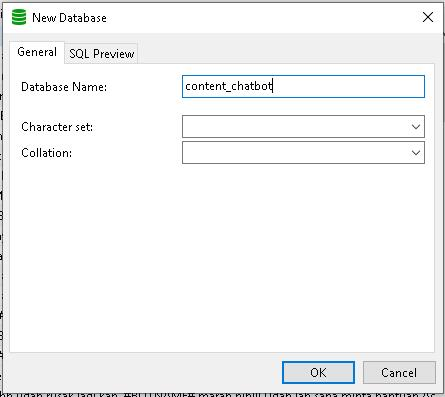
\includegraphics[scale=0.6]{26.5c.jpg}
        \newline
        d. Secara otomatis database yang  saya buat akan memiliki fitur untuk membuat table, view, backup, dan sebagainya. Disini saya memasukkan record saya untuk sementara.
        \newline
        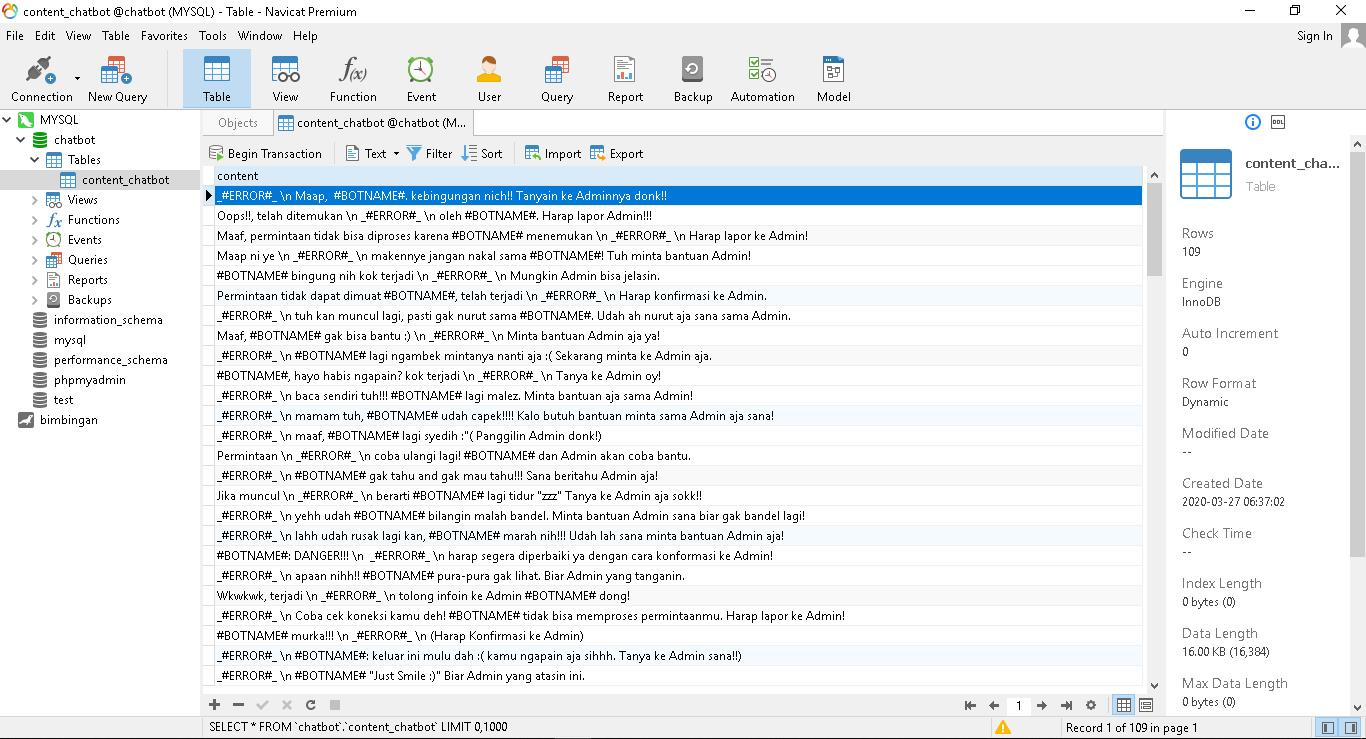
\includegraphics[scale=0.3]{26.5d.jpg}
        \newline
        \seti %harus diketik pada nomor terakhir
    \end{enumerate}


\section{Tanggal 28 Maret 2020:}
Kami telah menyelesaikan tugas pertama kami. Siang harinya, Bapak Rolly menjadwalkan pertemuan via google meet guna membahas cara menyambungkan navicat ke database mariadb. Setelah meeting dimulai, Bapak Rolly memberikan contoh bagaimana cara mengisi record. Sore harinya, Bapak Rolly meminta kami untuk merevisi kesalahan pada pekerjaan kami karena banyak dari kami yang mengerjakan pekerjaan kami yang belum sesuai dengan ketentuan Bapak Rolly. Berikut merupakan cara menghubungkan Navicat dengan database mariaDB
\newline
\newline
    \item 1. Mengisi SSH dengan ketentuan
        \begin{enumerate}
            \textbf{Name}  \textbf{=} \textbf{croot.ypbpi.or.id} \newline \textbf{Port} \textbf{=} 60606 \newline \textbf{User Name} \textbf{=} \textbf{if}
            \newline
            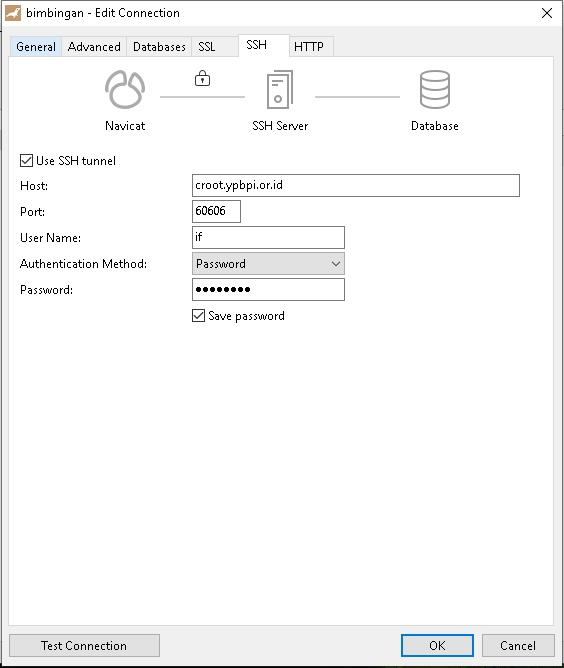
\includegraphics[scale=0.4]{28.1.jpg}
            \newline
            \seti %harus diketik pada nomor terakhir
        \end{enumerate}
    \item 2. Mengisi Database General dengan ketentuan        
            
        \begin{enumerate}
            \textbf{Connection} \textbf{=} bimbingan (bebas) \newline \textbf{Host} \textbf{=} \textbf{192.168.1.223} \newline \textbf{Port} \textbf{=} 3306 \newline \textbf{User Name} \textbf{=} \textbf{if}
            \newline
            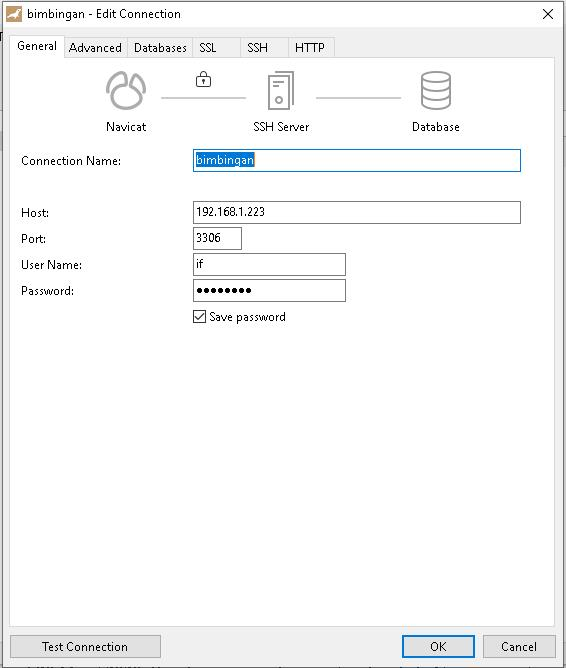
\includegraphics[scale=0.4]{28.2.jpg}
            \newline
            \seti %harus diketik pada nomor terakhir
        \end{enumerate}
    
        \item 3.	Setelah terhubung akan muncul “bimbingan” dengan 3 database yaitu information_schema, test, dan wanda.
            \newline
            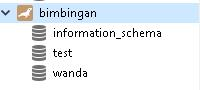
\includegraphics[scale=0.8]{28.3.jpg}
            \newline
        \item 4.	Selanjutnya yaitu mengisikan record yang telah dibuat ke dalam database wanda dengan cara kilik 2x pada database wanda lalu akan muncul beberapa table error_message, notfound_message, opening_message, dan waiting_message.
            \newline
            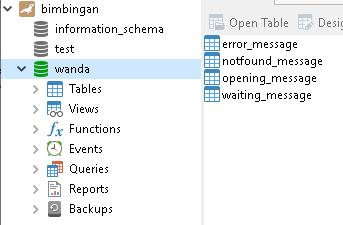
\includegraphics[scale=0.5]{28.5.jpg}
            \newline
        \item 5.	Pilih error\_message lalu masukkan record di dalam content.
            \newline
            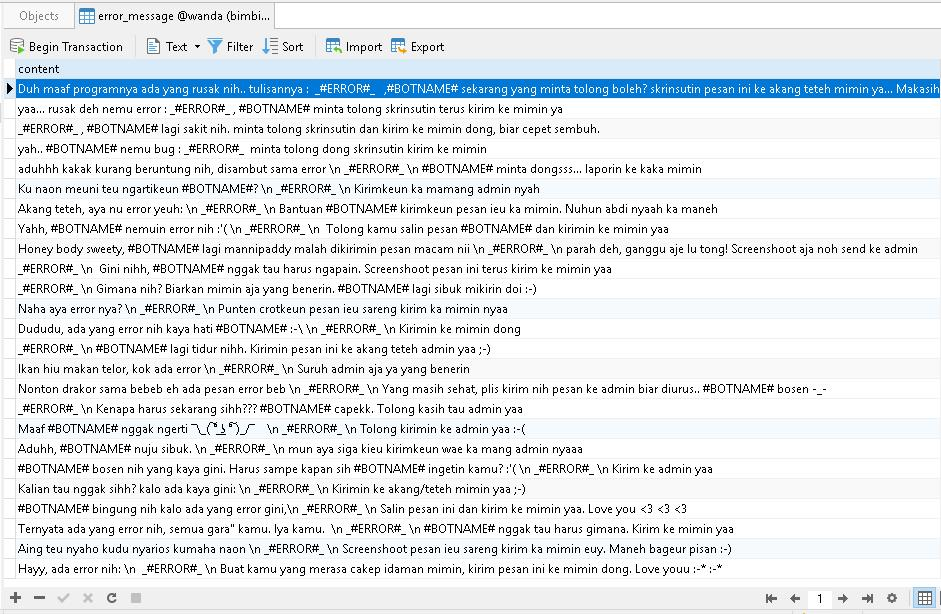
\includegraphics[scale=0.4]{28.4.jpg}
            \newline


\section{Tanggal 29 Maret 2020:}
Bapak menyarankan untuk memberi emoticon pada record kami. Kami menambahkan emoticon dan mengupdate record kami. Pada hari tersebut, Bapak Rolly merencanakan untuk melakukan pertemuan meeting lagi. Namun, karena ada beberapa hal, meeting tidak jadi dilaksanakan. Berikut merupakan beberapa contoh emoticon.
\newline
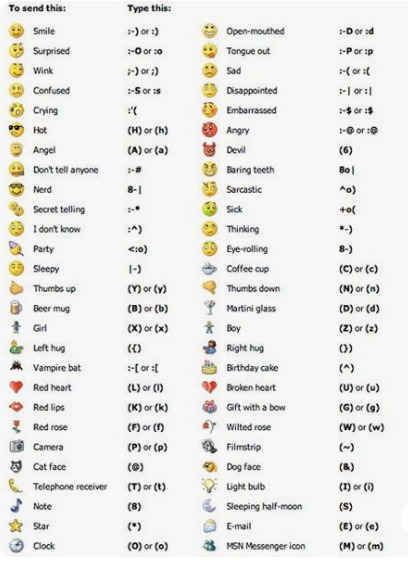
\includegraphics[scale=0.3]{29.1.jpg}
\newline
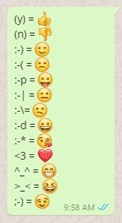
\includegraphics[scale=0.8]{29.2.jpg}
\newline


\section{Tanggal 30 Maret 2020:}
Bapak Rolly merencanakan untuk mengadakan meeting kembali. Namun, meeting tidak jadi dilaksanakan karena mungkin beberapa hal. 


\section{Tanggal 31 Maret 2020:}
Bapak Rolly memberikan tugas untuk mengisi opening_message. Pada hari tersebut, bapak menginformasikan bahwa pada proyek 1 setiap orang memegang 1 modul. Setiap orang 1 modul ekisting dan 1 modul pengembangan. Setelah itu, Bapak Rolly memberi tugas untuk mengisi record ke dalam waiting_message, yaitu antara lain kelas_mulai, kelas_selesai, dan jadwal_kelas sebanyak 34 record per orangnya.
    \newline
    \newline
        \item 1. opening\_message
            \newline
            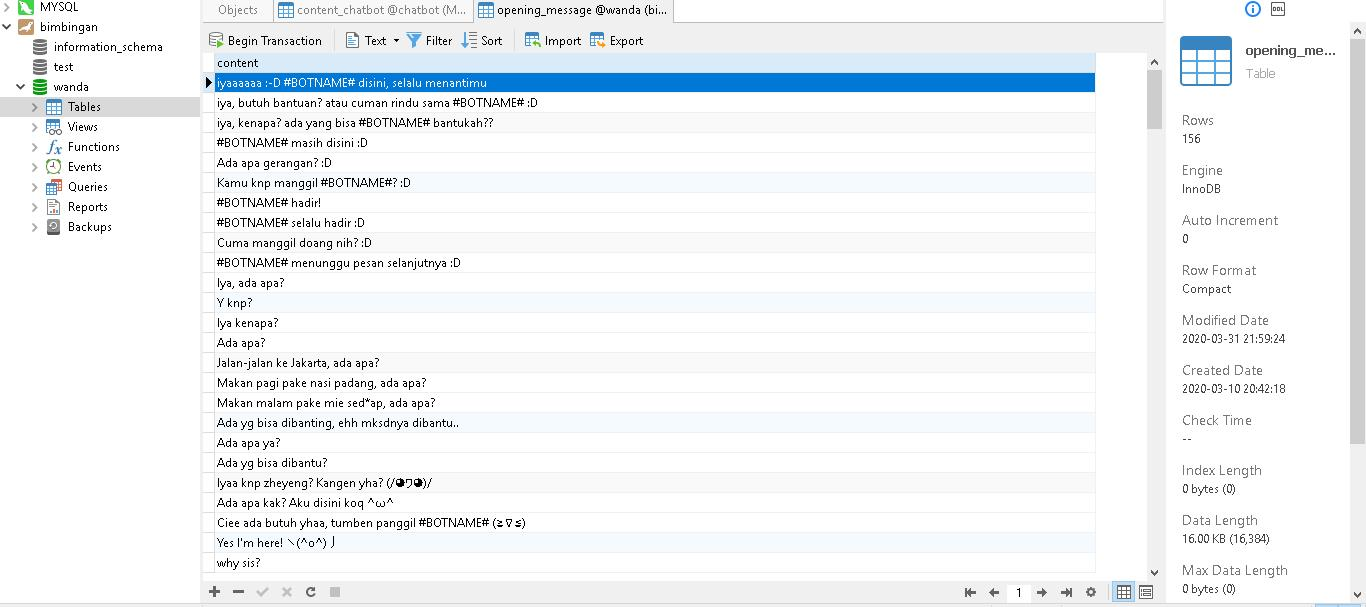
\includegraphics[scale=0.3]{31.1.jpg}
            \newline
        \item 2. kelas\_mulai
            \newline
            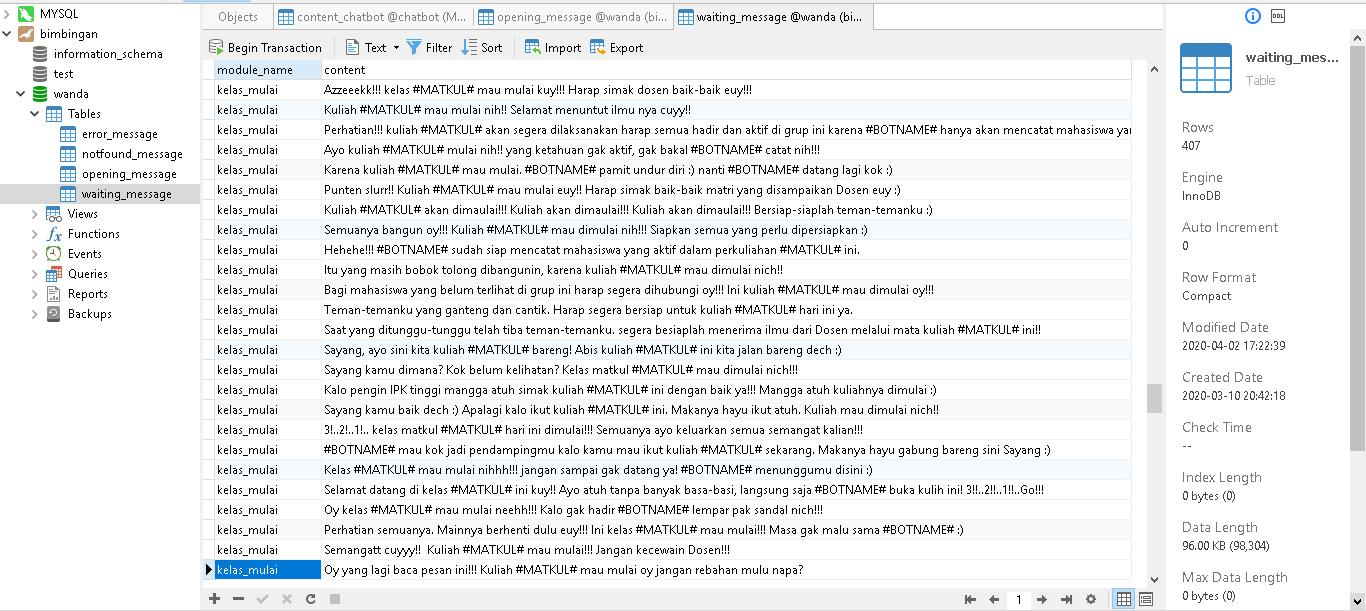
\includegraphics[scale=0.3]{31.2.jpg}
            \newline
        \item 3. kelas\_selesai
            \newline
            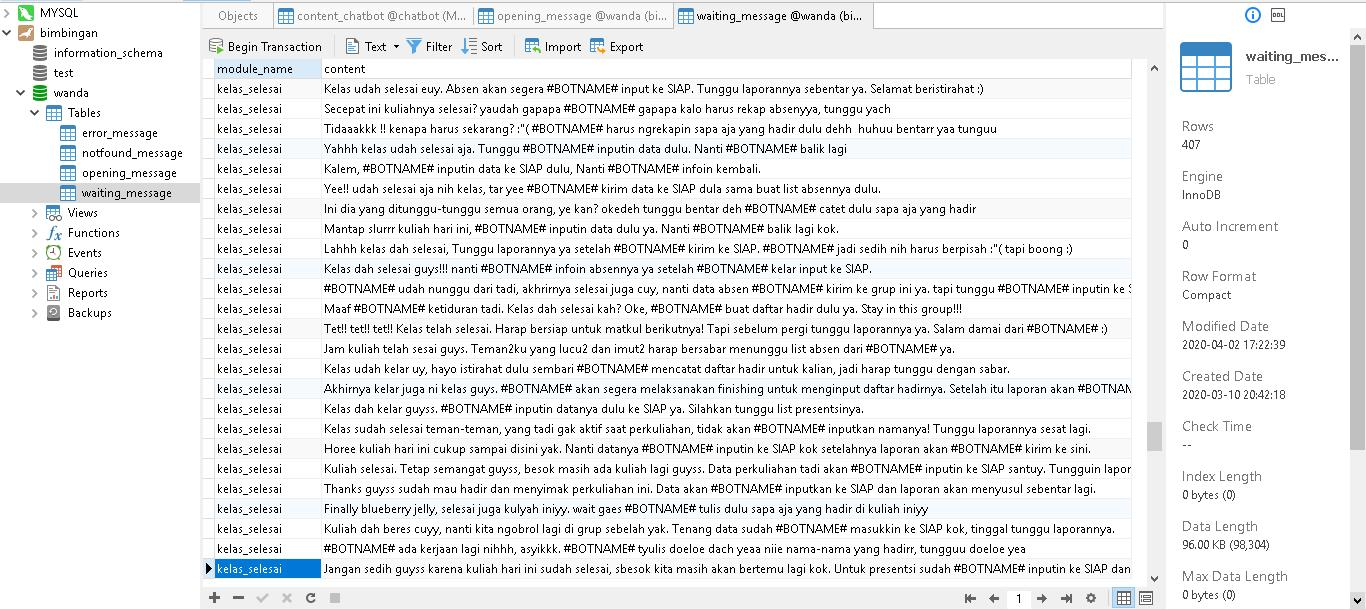
\includegraphics[scale=0.3]{31.3.jpg}
            \newline
        \item 4. jadwal\_kelas
            \newline
            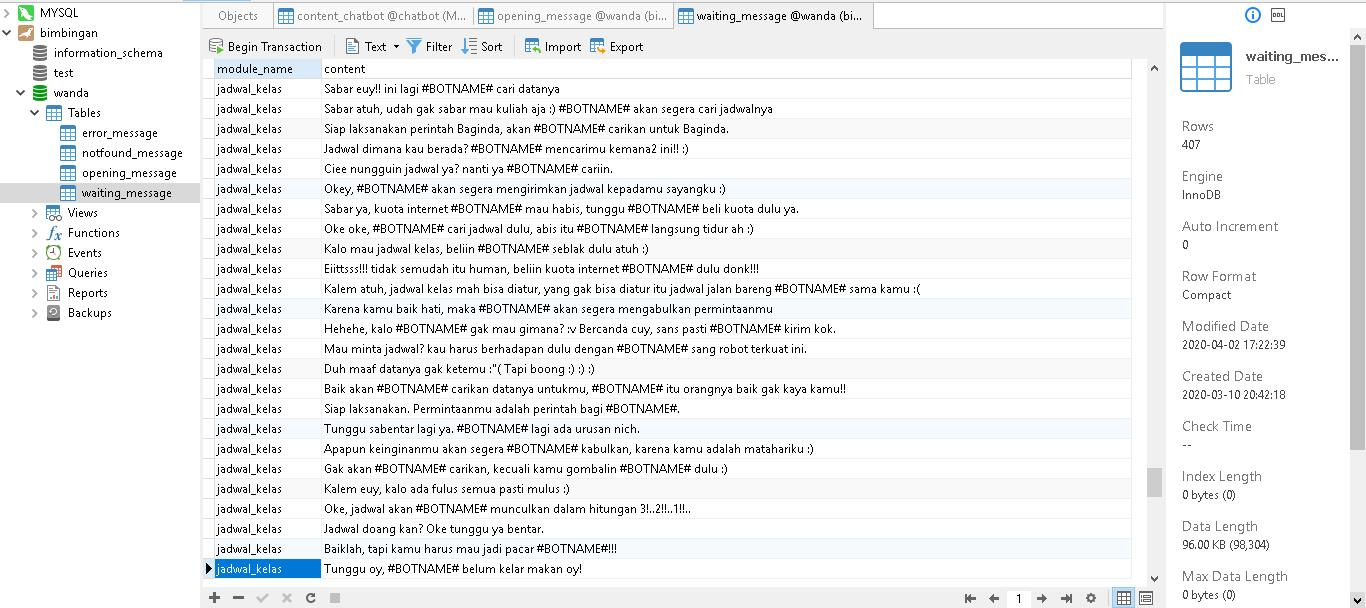
\includegraphics[scale=0.3]{31.4.jpg}
            \newline
            
    \item Penjelasan dari Tiap Table Database
    \newline
        \item 1. error_message
            \newline
            \par Tabel ini berfungsi untuk memberitahukan kepada pengguna bahwa terjadi kesalahan pada sistem (error system). Table error _message memiliki syarat yaitu harus memuat _#ERROR dan #BOTNAME#. Sebagai tambahan bisa memasukkan “\n” yang berfungsi sebagai baris baru (new line). Variable yang terdapat pada table yaitu _#ERROR#_ yang berfungsi menampilkan error yang terdapat pada aplikasi dan #BOTNAME# Merupakan variable yang berfungsi sebagai nama robot.
            \newline
        \item 2. notfound\_message
            \newline
            \par Table ini berfungsi untuk menjawab pesan yang tidak dapat diproses oleh robot. Jawaban yang diberikan oleh robot disesuaikan dengan bahasa sehari-hari manusia sehingga tidak terlihat seperti robot. Table ini hanya memiliki syarat harus memuat #BOTNAME# sebagai nama robotnya. Variable yang terdapat pada table yaitu #BOTNAME# Merupakan variable yang berfungsi sebagai nama robot.
            \newline
        \item 3. opening\_message
            \newline
            \par Tabel  ini merupakan pesan respon  yang disampaikan robot karena telah menyebutkan nama robot. Variable yang terdapat pada table yaitu #BOTNAME# Merupakan variable yang berfungsi sebagai nama robot.
            \newline
        \item 4. waiting\_message
            \newline
            \par Tabel ini merupakan table yang berisi respon kepada pengguna untuk menunggu. Tabel ini memuat kelas_mulai, kelas_selesai, jadwal_kelas. Variable yang terdapat pada table yaitu #BOTNAME# Merupakan variable yang berfungsi sebagai nama robot.
            \newline
            \newline
        \item a. kelas\_mulai
            \newline
            \par Tabel ini merupakan pemberitahuan bahwa perkuliahan suatu mata kuliah akan segera dimulai. Tabel ini memiliki syarat yaitu harus memuat #BOTNAME# dan #MATKUL#. Variable yang terdapat pada table yaitu #BOTNAME# Merupakan variable yang berfungsi sebagai nama robot dan #MATKUL# Merupakan variable yang berfungsi sebagai mata kuliah yang akan dilaksanakan
            \newline
        \item b. kelas\_selesai
            \newline
            \par Tabel ini merupakan pemberitahuan bahwa perkuliahan suatu mata kuliah sudah berakhir. Tabel ini memiliki syarat yaitu harus memberitahukan kepada pengguna bahwa robot akan menginputkan data ke SIAP dan mengirimkan laporannya ke grup tersebut. Variable yang terdapat pada table yaitu #BOTNAME# Merupakan variable yang berfungsi sebagai nama robot.
            \newline
        \item c. jadwal\_kelas
            \newline
            \par Tabel ini merupakan respon robot ketika pengguna meminta jadwal. robot akan mengirimkan jadwal ke grup tersebut ketika pengguna menggunakan kata kunci “jadwal kelas”. Variable yang terdapat pada table yaitu #BOTNAME# Merupakan variable yang berfungsi sebagai nama robot.
            \newline

\section{Tanggal 1 April 2020:}
Bapak Rolly memberikan instruksi untuk belajar git dan selenium untuk website modul pengembangan. Dan akan dipandu oleh Kak Wahyu dan Kak Inal. Berdasarkan modul yang telah diberikan kami mengikuti langkah-langkah sebagai berikut:
    \newline
    \newline
        \item 1.	Download dan install  Gitbash lalu membuat akun Github
            \newline
            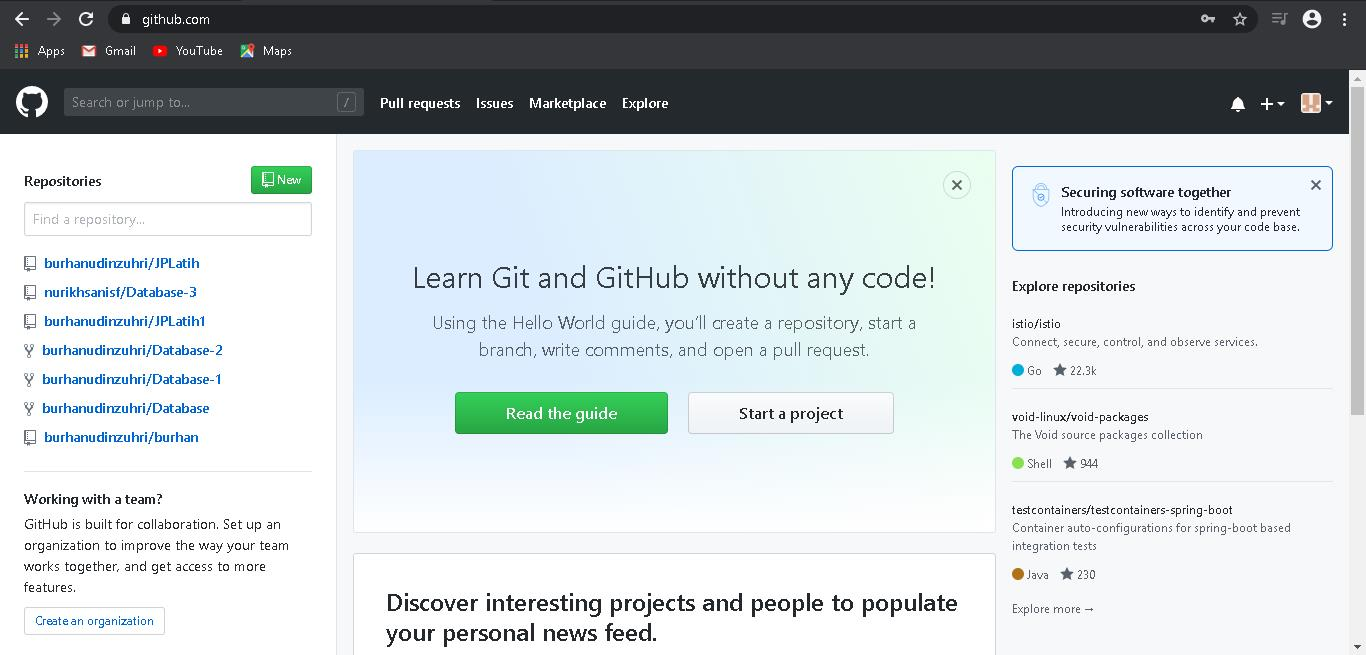
\includegraphics[scale=0.3]{32.1.jpg}
            \newline
        \item 2.	Membuat akun GitLab, namun berhubung GitLab sudah terhubung dengan Github maka tidak perlu membuat akun, dan hanya sign in saja.
        \newline
            \item 3.	Konfigurasi Key
                \newline
            \item a. Buka Gitbash di home directory lalu ketik “cd” lalu Enter
                \newline
                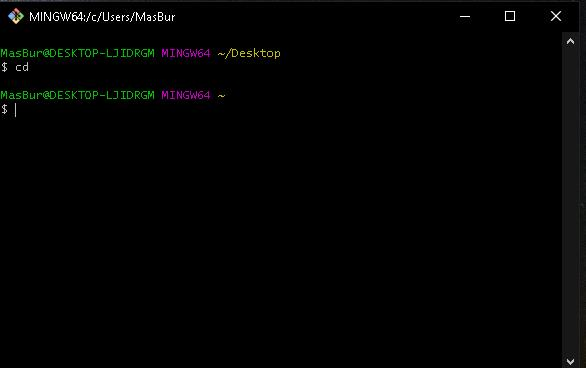
\includegraphics[scale=0.5]{32.3a.jpg}
                \newline
            \item b. Ketik “ssh-keygen –t rsa –b 4096 –C “burhanudinzuhri25@gmail.com” (isi sesuai email anda)” dan  di perintah keygen ini, cukup dengan klik enter-enter saja.
                \newline
                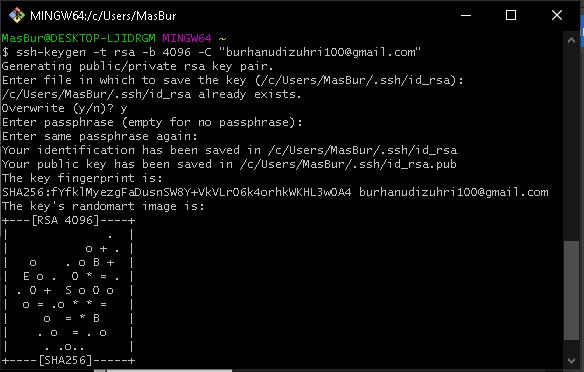
\includegraphics[scale=0.5]{32.3b.jpg}
                \newline
            \item c. Masukkan perintah “cat . ssh/id_rsa .pub” maka akan keluar hasilnya seperti ini
                \newline
                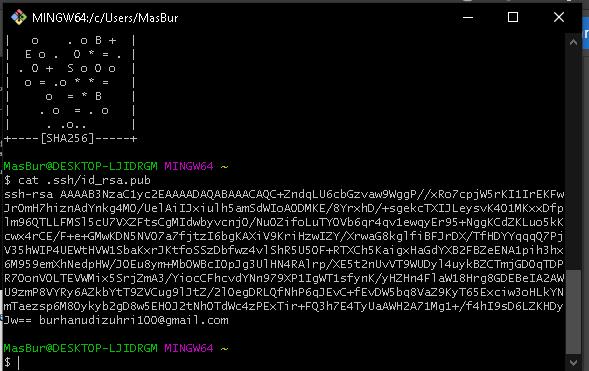
\includegraphics[scale=0.5]{32.3c.jpg}
                \newline
            \item d. Selanjutnya masuk kea kun Github, klik Menu Setting, pilih menu SSH and GPG keys dan tambahkan New SSH key
                \newline
                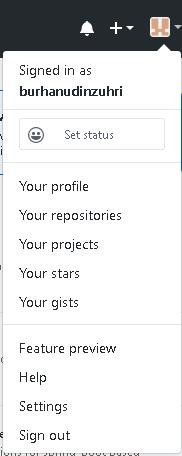
\includegraphics[scale=0.5]{32.3d.jpg}
                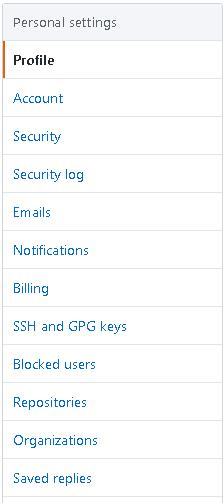
\includegraphics[scale=0.45]{32.3e.jpg}
                \newline
                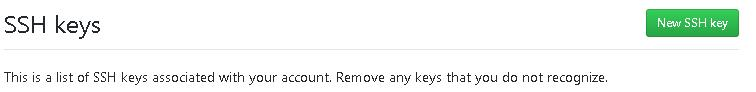
\includegraphics[scale=0.5]{32.3f.jpg}
                \newline
    
    \item Penjelasan Git
    \newline
        \item 1. Git
            \newline
            Git adalah alat yang digunakan untuk mengembangkan sebuah project secara online
            \newline
        \item 2. ssh-keygen –t rsa –b 4096 -C “burhanudinzuhri25@gmail.com
            \newline
            Perintah untuk menghasilkan key SSH dari computer.
            \newline
        \item 3. cat . ssh/id_rsa .pub
            \newline
            Perintah untuk menampilkan key SSH.
            \newline



\section{Tanggal 2 April 2020:}
Bapak Rolly memberikan tugas untuk membuat laporan pekerjaan harian di excel dan menarketkan 4 tugas yaitu:
    \newline
    \newline
        \item 1.	Membuka website memakai selenium dan kode programnya di push ke repo masing-masing dengan syarat setiap orang membuka website yang berbeda.
            \newline
        \item 2.	Menginsertkan record masing-masing tabel 34 row.
            \newline
        \item 3.	Memasukkan laporan pada Github dan mengupdatenya di README.md
            \newline
        \item 4.	Memberitahu Bapak Rolly jika tugas sudah selesai dikerjakan. 
            \newline
        
        \item 1.	Untuk tugas website selenium kami menginstall Anaconda dan mengunduh Chrome Driver.
        Berikut merupakan langkah-langkah mengerjakan tugas selenium
            \newline
        a. Mendownload dan menginstall Anaconda sesui versi masing-masing.
            \newline
            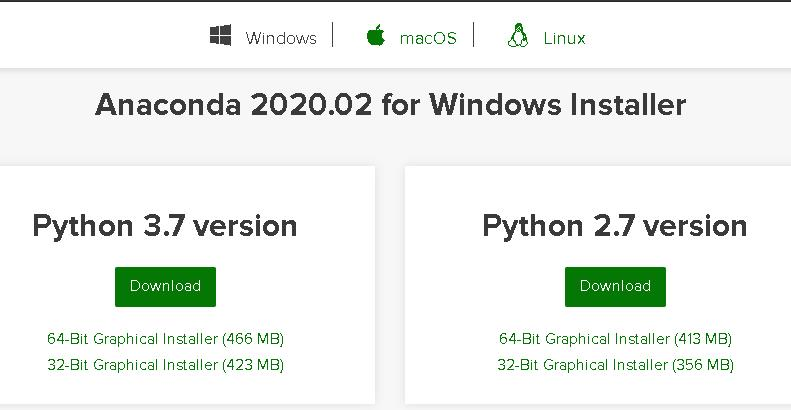
\includegraphics[scale=0.5]{33.1a.jpg}
            \newline
        b. Mendownload Chromedriver dan meletakkannya di C:/Windows/System32
            \newline
            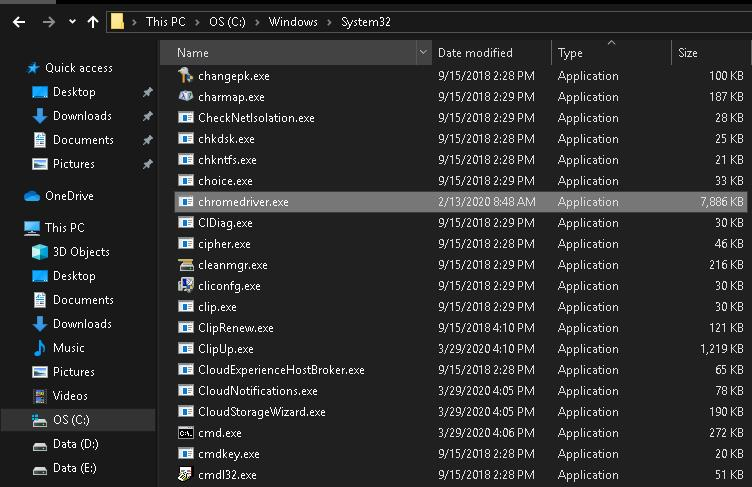
\includegraphics[scale=0.5]{33.1b.jpg}
            \newline
        c. Menginstall selenium menggunakan cmd (Command Prompt) dengan mengetik “pip install selenium”
            \newline
            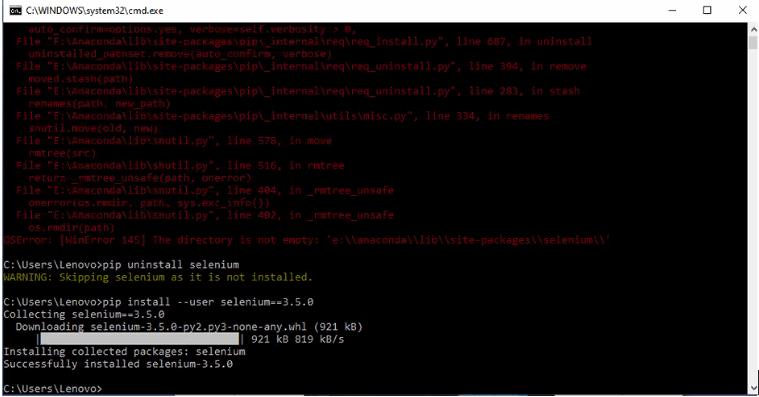
\includegraphics[scale=0.5]{33.1c.jpg}
            \newline
        d. Membuka Spyder/Visual Studio Code yang sudah terinstall bahasa pemrograman python dan memasukan perintah sebagai berikut
        \newline
            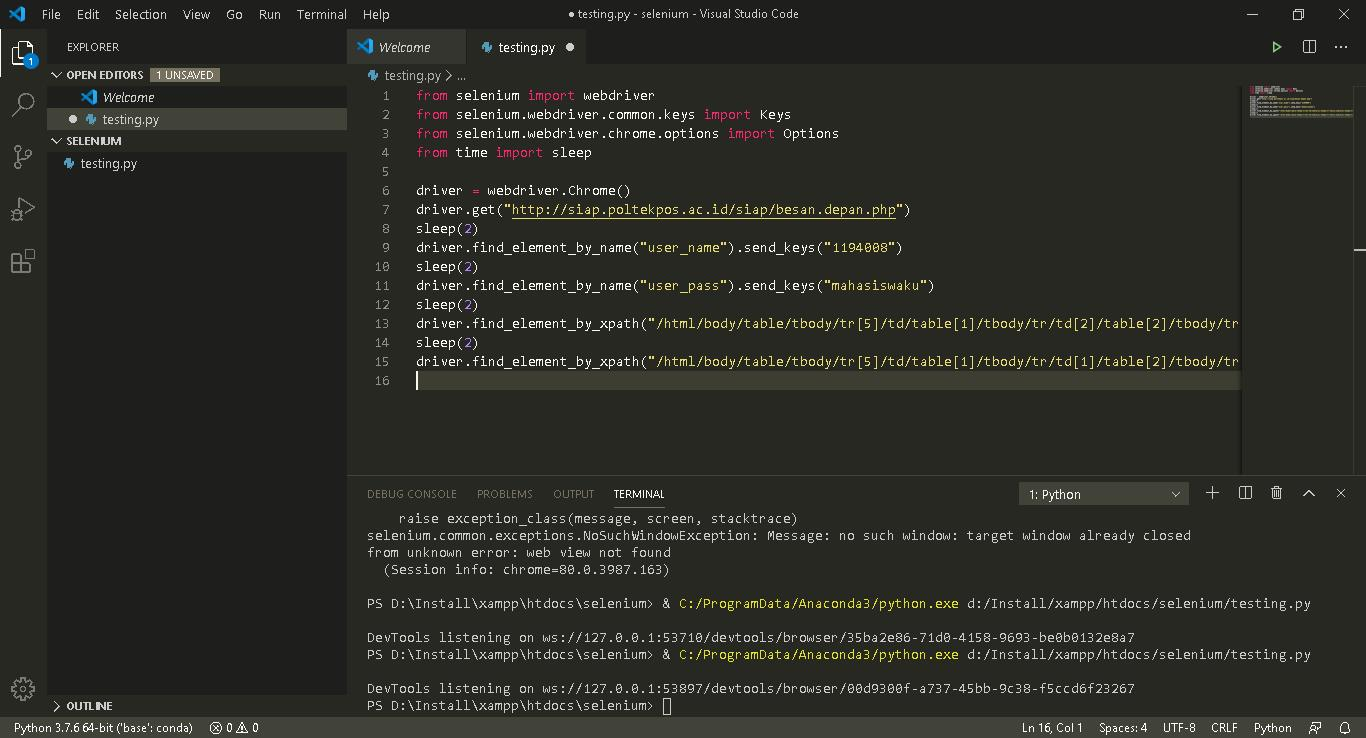
\includegraphics[scale=0.3]{33.1d.jpg}
            \newline
            from selenium import webdriver
            \newline
            from selenium.webdriver.common.keys import Keys
            \newline
            from selenium.webdriver.chrome.options import Options
            \newline
            from time import sleep
            \newline
            \newline
            driver = webdriver.Chrome()
            \newline
            driver.get("http://siap.poltekpos.ac.id/siap/besan.depan.php")
            \newline
            sleep(2)
            \newline
            driver.find_element_by_name("user_name").send_keys("1194008")
            \newline
            sleep(2)
            \newline
            driver.find_element_by_name("user_pass").send_keys("xxxxxxxxxxx")
            \newline
            sleep(2)
            \newline
            driver.find_element_by_xpath("/html/body/table/tbody/tr[5]/td/table[1]/tbody/tr/td[2]/table[2]/tbody/tr[1]/td[2]/div/form/input[4]").click()
            \newline
            sleep(2)
            \newline
            driver.find_element_by_xpath("/html/body/table/tbody/tr[5]/td/table[1]/tbody/tr/td[1]/table[2]/tbody/tr[1]/td[2]/a[2]").click()
            \newline
            \newline
            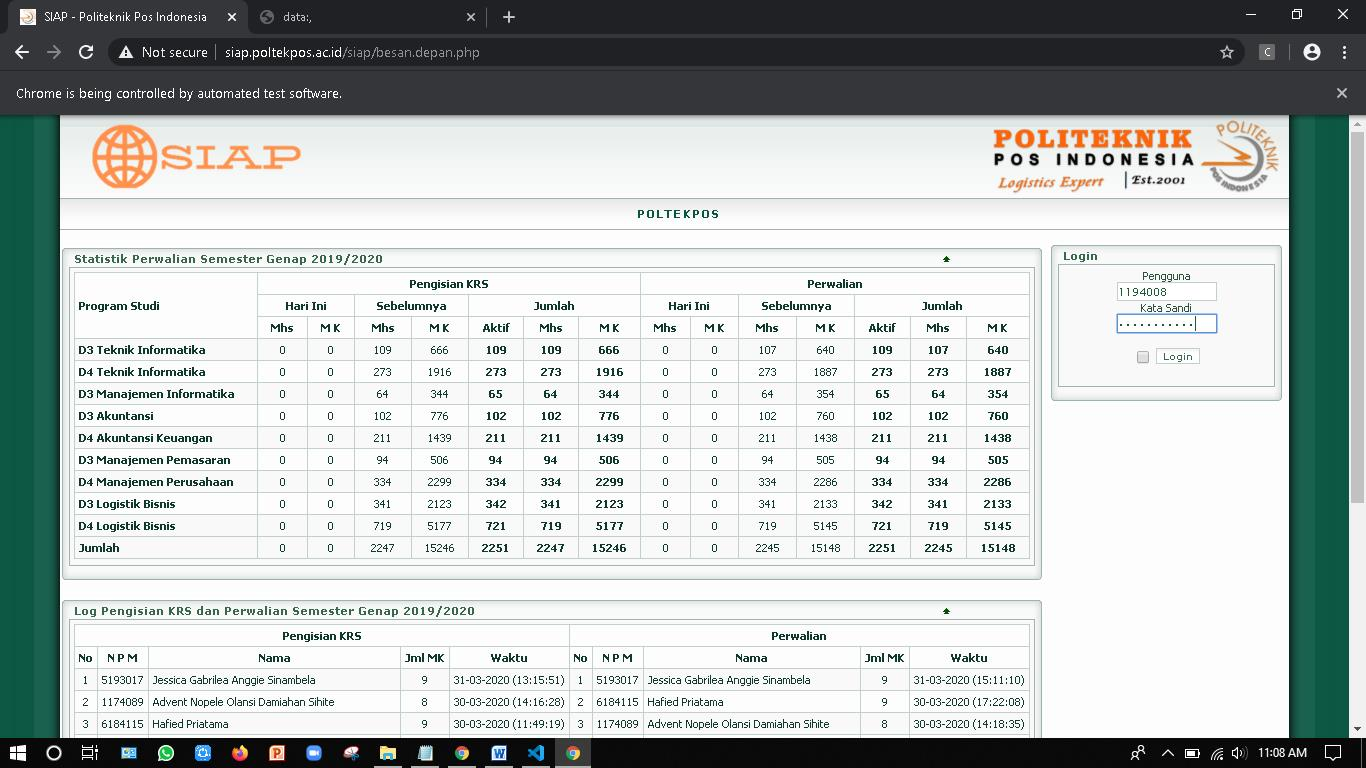
\includegraphics[scale=0.3]{33.1e.jpg}
            \newline
        \item 2. Untuk tugas menginsertkan record masing-masing tabel 34 row kami mengisikan ke 6 table yang tersedia yaitu error_message, notfound_message, opening_message, kelas_mulai, kelas_selesai, dan jadwal_kelas.
            \newline
            \newline
        \item 3.	Memasukkan file selenium yang telah dibuat dan laporan pada Github dan mengupdatenya di README.md
           \newline
            \item a. Buat folder baru lalu klik kanan pilih “Gitbash Here”	
                \newline
                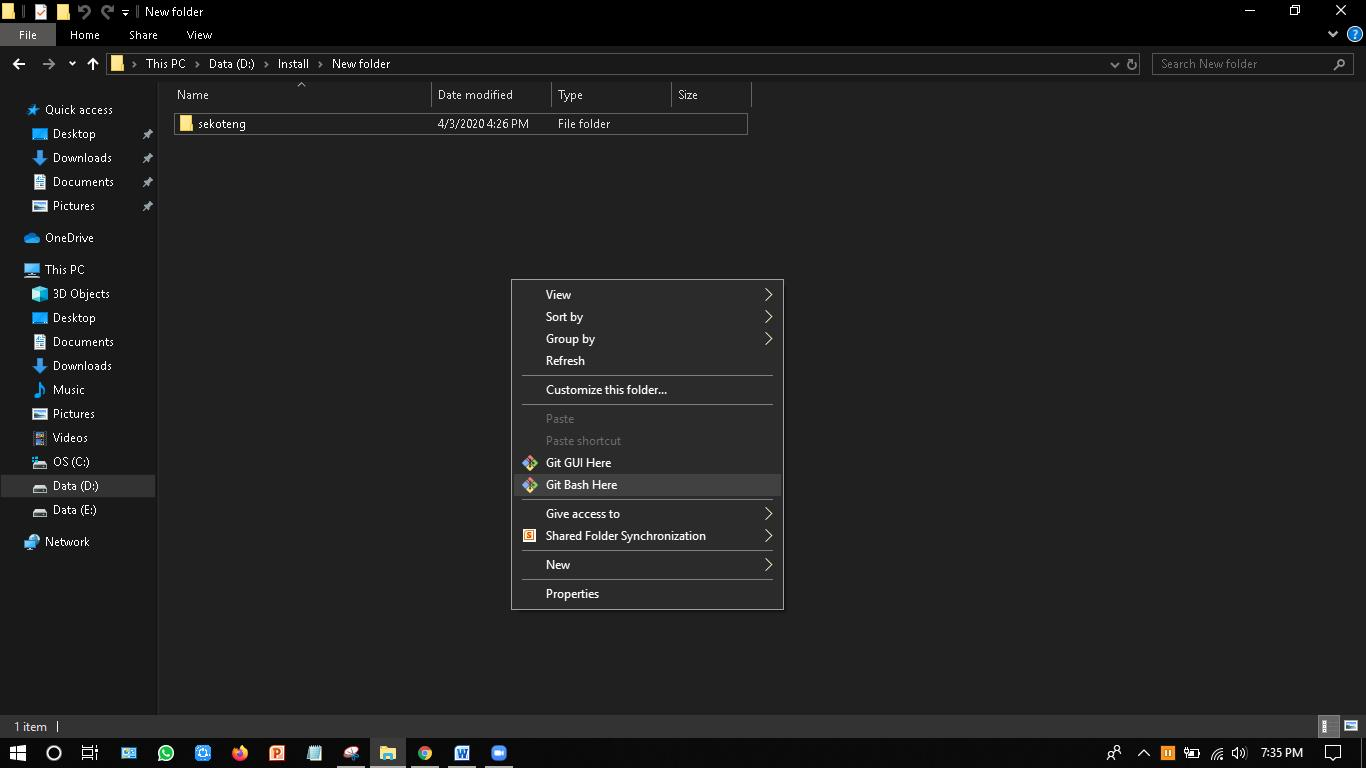
\includegraphics[scale=0.3]{33.3a.jpg}
                \newline
            \item b. Buka Github dan pilih repository, lalu clone dan cpy URLnya
                \newline
                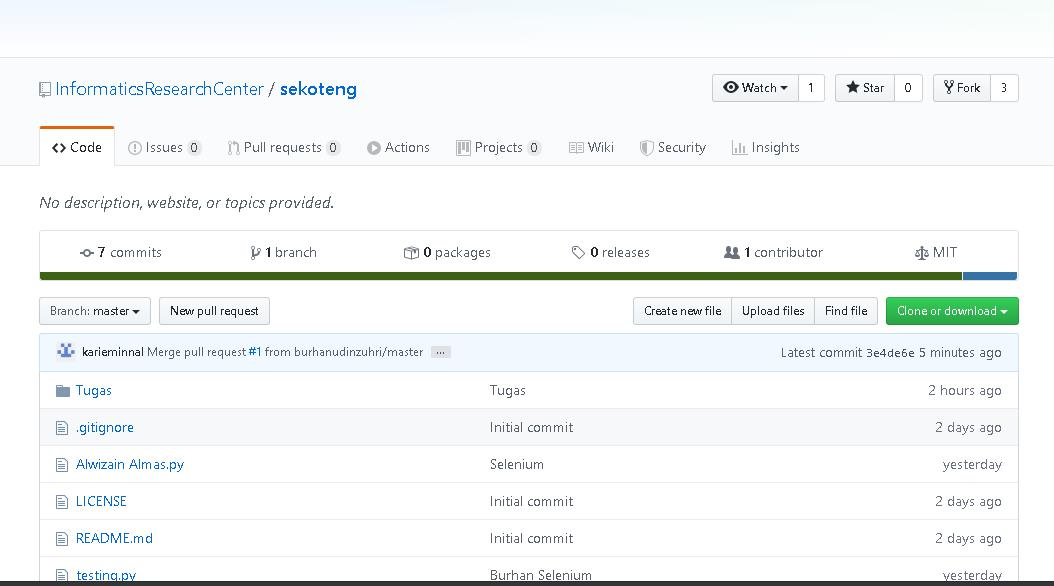
\includegraphics[scale=0.3]{33.3b.jpg}
                \newline
            \item c. Masukkan perintah “git clone https://github.com/InformaticsResearchCenter/sekoteng.git”
                \newline
                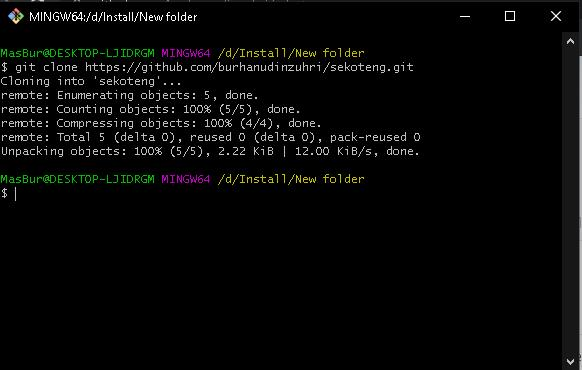
\includegraphics[scale=0.4]{33.3c.jpg}
                \newline
            \item d. Setelah selesai maka akan muncul folder baru dengan nama sesui repository, kemudian masukkan file tersebut.
                \newline
                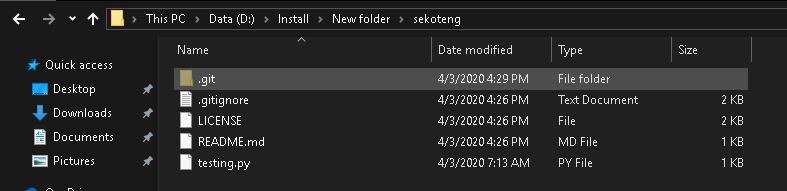
\includegraphics[scale=0.5]{33.3d.jpg}
                \newline
            \item e. Klik kanan pada halaman dan pilih Gitbash dan tambahkan perintah seperti dibawah ini
                \newline
                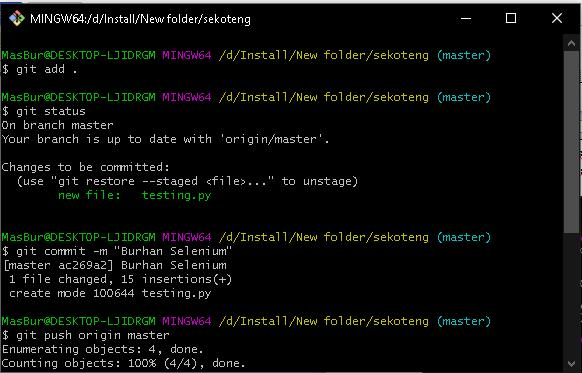
\includegraphics[scale=0.4]{33.3e1.jpg}
                \newline
                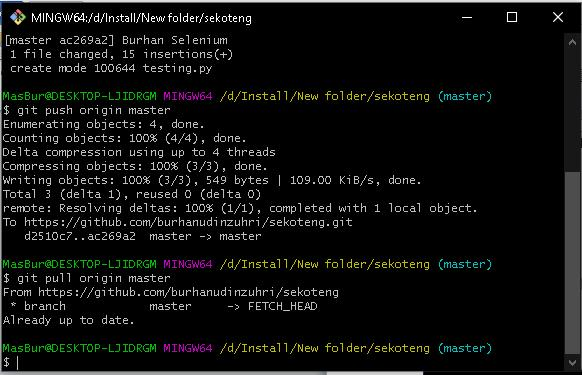
\includegraphics[scale=0.4]{33.3e2.jpg}
                \newline
            \item f. Cek kembali file yang tadi diupload dan pull request
                \newline
                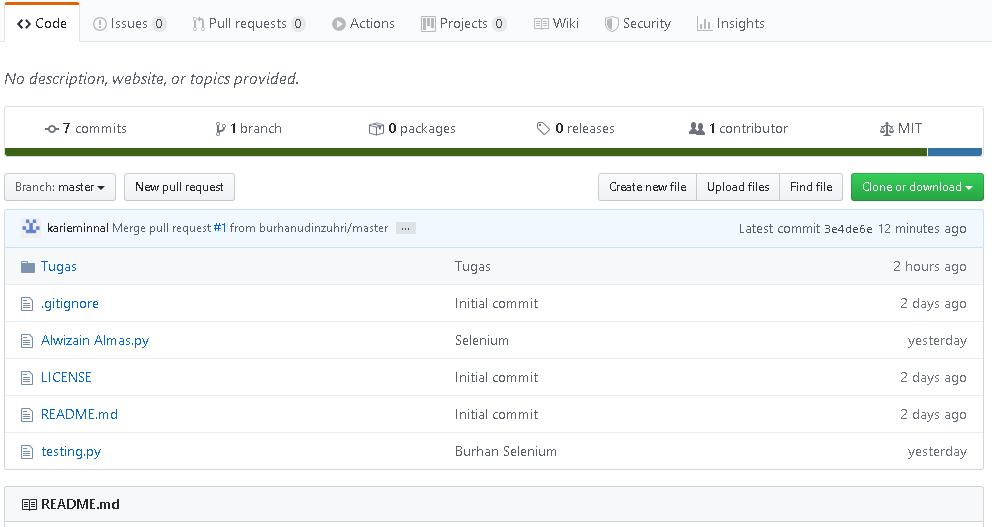
\includegraphics[scale=0.4]{33.3f.jpg}
                \newline


\end{document}